% Project Specification
\begin{figure*}[t]
  \begin{minipage}[t]{0.33\textwidth}
    \centering
    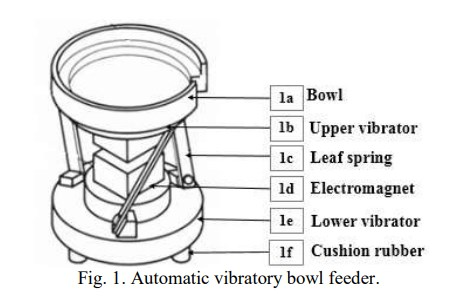
\includegraphics[width=\textwidth,height=5cm, keepaspectratio]{imgs/articles/feeder.jpg}
    \caption{VBF\cite{nam2019design}}
    \label{fig:feeder}
  \end{minipage}
  \hfill
  \begin{minipage}[t]{0.33\textwidth}
      \centering
      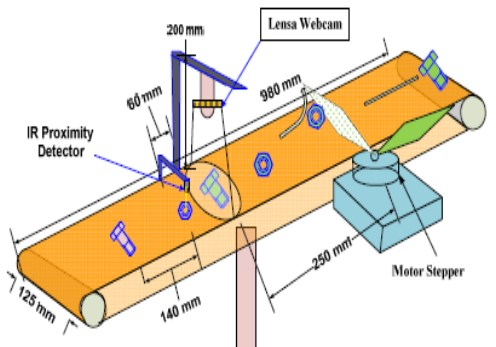
\includegraphics[width=\textwidth,height=5cm, keepaspectratio]{imgs/articles/conveyor.jpg}
      \caption{Conveyor Belt\cite{Dhenge2013MechanicalNS}}
      \label{fig:conveyor}
      \end{minipage}
  \hfill
  \begin{minipage}[t]{0.33\textwidth}
    \centering
    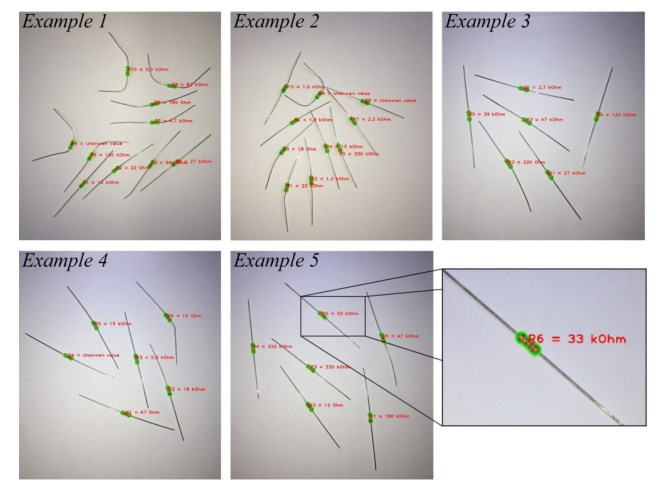
\includegraphics[width=\textwidth,height=5cm, keepaspectratio]{imgs/articles/resistordata.jpg}
    \caption{Resistor Test Set\cite{8939034}}
    \label{fig:resistordata}
  \end{minipage}
\end{figure*}

\section{Project Specification}
\label{sec:project-specification}
The motivation for this project is three-fold; to solve the problem of electronic waste and cluttered workspaces in the Level 1 Labs;
to alleviate the time-consuming process of sorting electronic components from the Labs' technicians; and 
to bring the Lab closer to meeting the requirements for the LEAF (Laboratory Efficiency Assessment Framework) certification\cite{leaf} that
the Lab is currently working towards.

The LEAF certification is a framework that aims to improve the efficiency of laboratories by reducing waste, energy consumption, and costs.
This project aligns with the LEAF certification's goals by reducing the amount of electronic waste produced by the Lab.

The project aims to achieve these goals by employing state-of-the-art computer vision techniques to classify various electronic components,
and then sort them into designated bins. The project's deliverables are as follows:
\begin{mylist}
  \item A computer vision system for component identification
  \item An interface from which to observe and control the system's state
  \item A semi-automated sorting mechanism
  \item Potentially, full automation of the sorting process or additional features like IC testing
\end{mylist}
\noindent
After an initial consultation with Dr. Stott and visiting the Level 1 Labs to discuss the project,
samples of the different electrical components commonly used were received, as follows:
\begin{multicols}{2}
  \begin{mylist}
    \item Resistors
    \item Capacitors
    \item Ceramic Capacitors
    \item Inductors
    \item Diodes
    \item MOSFETs
    \item Transistors
    \item LEDs
    \item Wires
    \item ICs
  \end{mylist}
\end{multicols}

\noindent
For this initial stage of the project, the focus is on developing the foundation of the system that the project
will be built upon so that the development of the various systems can be done independently, in parallel, and in such a way that each system
is modular and easily extensible. For this reason, the project was initially split into three stages:
\begin{mylist}
  \item Initial development of a computer vision system for component identification
  \item Integration of a semi-automated sorting mechanism
  \item Potentially, full automation of the sorting process or additional features like IC testing
\end{mylist}
After the initial stage, it was decided that the first stage would be split into two stages, with the first stage focusing on the development of the foundation of the system, 
and the second stage focusing on the development of the computer vision system, for a total of four stages. This was because the development of the foundation of the
system took longer than expected, and the vision system needs to be trained on data that is representative of the conditions it will be used in, which requires the mechanical design to be finalised.

This approach was adopted to establish defined goals, ensuring that the project consistently progresses towards a deliverable product. 
Each stage extends the previous stage, so the project can be considered as a series of smaller projects. 
